\section{Results}
\label{sec:28}

\subsection{Summary}
Each of the measures showed a good bit of variability between imaging sites (see Figure 1 for an example plot showing standardized DVARS for ABIDE). Ranks calculated from the weighted average of standardized quality metrics indicated that CMU? was the worst performing site and NYU? was the best. QI1 and SNR were the best predictors of manually applied structural data quality scores, and EFC, FWHM, Percent FD, and GSR were all significant predictors of functional data quality (fig 2, $p < 0.0001$). A few of the measures are highly correlated (fig. 3) such as SNR, CNR and FBER, which measure very similar constructs, indicated that there is some room for reducing the set of measures. For the functional data, the test­-retest reliability of several of the spatial measures of quality were very high (fig 4., EFC, FBER, GSR) reflecting their sensitivity to technical quality (i.e. MR system and parameters) whereas temporal measures were lower reflecting their sensitivity to physiological factors such as head motion. Similarly in the structural data, it appears that measures can be divided into those that are more sensitive to technical quality (EFC, FWHM) and those that favor physiological variation (CNR, QI1) based on test­-retest reliability.

\subsection{Correlations between measures}
We notice that anatomical measures more correlated each other than functional measures, and correlations between measures in ABIDE are similar to correlations in CoRR.

\begin{table}[ht!]
\textbf{\refstepcounter{table}\label{tab_anat_cor} Table \arabic{table}.}{ Correlations between anatomical measures. CoRR in the upper triangular, ABIDE in the lower triangular. *indicates p-value less than 0.05 }
\processtable{}
{\begin{tabular}{ l c c c c c c p{1.5cm}}\\
        \hline
         Anatomical & CNR & EFC & FBER & FWHM & Qi1 & SNR \\
        \hline
        CNR &  & -0.506* & 0.316* & -0.111 & -0.489* & 0.733* \\
        EFC & -0.458* &  & -0.126 & -0.151 & 0.572* & -0.562* \\
        FBER & 0.436* & -0.286* & & -0.038 & -0.197 & 0.444* \\
        FWHM & -0.056 & 0.109 & 0.056 & & -0.082 & -0.137 \\
        Qi1 & -0.392* & 0.372* & -0.238 & 0.073 & & -0.549* \\
        SNR & 0.760* & -0.61* & 0.675* & -0.112 & -0.448* & \\
        \hline
        \end{tabular}}{}
\end{table}

\begin{table}[h]
  \begin{center}
    \begin{tabular}{ l c c c c c c c c p{1.5cm}}
    \hline
    Functional & EFC & FBER & FWHM & SNR & DVARS & Mean RMSD & Quality & GCOR  \\ \hline
    EFC & & -0.264* & 0.140 & -0.707* & -0.036 & -0.007 & -0.820 & -0.056 \\
    FBER & -0.134 & & 0.053 & 0.838* & 0.100 & 0.070 & 0.290* & 0.017 \\
    FWHM & -0.023 & 0.168 & & -0.036 & -0.175 & 0.013 & -0.030 & -0.021 \\
    SNR & -0.586* & 0.845* & 0.118 & & -0.047 & 0.070 & 0.624* & 0.043 \\
    DVARS & 0.012 & 0.015 & -0.108 & -0.016 & & -0.020 & -0.116 & 0.197 \\
    Mean FD & -0.029 & 0.129 & 0.143 & 0.139 & -0.140 & & 0.162 & -0.014 \\
    Quality & -0.693* & 0.234 & 0.106 & 0.531 & -0.153 & 0.310* & & -0.042 \\
    GCOR & -0.098 & 0.066 & 0.035 & 0.092 & 0.207 & 0.060 & 0.046 & \\
    \hline
    \end{tabular}
  \end{center}
%  \caption{Correlations of functional measures; CoRR in the upper triangular, ABIDE in the lower triangular. * indicates p-value less than 0.05}
\end{table}

\subsection{Test-retest of the measures (for CoRR)}
Figure 3 shows the boxplots of ICCs of each site for each measure. Note that variances of ICCs of functional measures are less than of anatomical measures. EFC, FBER, SNR, Percent FD for functional measures have very high ICCs average over 0.75 while ICC of EFC for anatomical is average over 0.75

\subsection{Relationship of measures with hand assessments}
Table 2 summarizes the results. Figure 4 shows boxplots of most discriminative measures vs. hand assessments. CNR, QI1, SNR are significant predictors of hand assessment in anatomical while all measures except FBER, SNR are significant in functional.

\begin{table}
\textbf{\refstepcounter{table}\label{tab_log_reg_anat} Table \arabic{table}.}{ Logistic regression results --- Anatomical }
  \begin{center}
    \begin{tabular}{ l r r r p{1.2cm} }
    \hline
    Measure  &Estimate & Std Err & p-value  \\ \hline
    CNR	&	0.370	&	0.058	&	0.000	\\
    EFC	&	2.463	&	2.369	&	0.298	\\
    FBER&	0.002	&	0.001	&	0.009	\\
    FWHM&	0.083	&	0.126	&	0.513	\\
    Qi1	&	-7.484	&	1.064	&	0.000	\\
    SNR	&	-0.179	&	0.039	&	0.000	\\
    \hline
    \end{tabular}

  \end{center}
\end{table}

\begin{table}
  \textbf{\refstepcounter{table}\label{tab_log_reg_func} Table \arabic{table}.}{ Logistic regression results --- Functional }
  \begin{center}
    \begin{tabular}{ l r r r }
    \hline
    Measure &Estimate & Std Err & p-value  \\ \hline
    EFC	    &	7.136	&	2.823	&	0.011	\\
    FBER	&	-0.041  &	0.020	&	0.043	\\
    FWHM	&	1.864	&	0.326	&	0.000	\\
    SNR	    &	0.369	&	0.145	&	0.011	\\
    Quality	&	4.846	&	3.434	&	0.158	\\
    RMSD	&	-2.139  &	0.480	&	0.000	\\
    DVARS	&	1.809	&	0.754	&	0.016	   \\
    GCOR	&	3.789	&	1.016	&	0.000	\\
    \hline
    \end{tabular}
  \end{center}
\end{table}


\subsection{Relationship of measures with scanning parameters}

\begin{table}
  \textbf{\refstepcounter{table}\label{anat_spat_reg} Table \arabic{table}.}{ Anatomical spatial - Regression analysis for the relationship of measures with scanning parameters. Estimated coefficients of each parameter are reported by measures. * indicates p-value less than 0.05.  }
  \begin{center}
    \begin{tabular}{ l l r r r r r r }
    \hline
    Parameter / measure & & CNR & EFC & FBER & FWHM & Qi1 & SNR \\ \hline
    Intercept & & -153.400 & 1.568* & -8160.880 & -11.093 & 0.956 & -116.510 \\
    Scanner & GE MR750 & 11.463 & -0.082 & 1977.000 & -8.292 & -0.030 & -20.262 \\
     & GE Sig & -4.534 & -0.124 & 643.650 & 1.379 & -0.188 & 21.553 \\
     & Phillips Achieva & 45.799* & -0.383* & 2386.040 & 9.017 & -0.174 & 55.190 \\
     & Phillips Intera & 15.405* & -0.146* & 410.430 & -0.819 & -0.168* & 11.042 \\
     & Siemens Allegra & 15.587 & -0.044 & 2564.100 & -7.555 & -0.270* & -15.226 \\
     & Siemens Tim TRIO & 4.096 & -0.020 & 1110.120 & -4.282 & -0.213* & -15.063 \\
     & Siemens Verio & 0.000 & 0.000 & 0.000 & 0.000 & 0.000 & 0.000 \\
    Slice Gap & 0 & 5.776 & -0.037 & 232.290 & 2.314 & 0.063 & 11.518 \\
     & 1 & 0.000 & 0.000 & 0.000 & 0.000 & 0.000 & 0.000 \\
    Slice Acquisition & int+ & 0.000 & 0.000 & 0.000 & 0.000 & 0.000 & 0.000 \\
     & seq+ & -2.640 & 0.215 & 1848.390 & -11.416 & -0.060 & -39.822 \\
     & seq- & 0.000 & 0.000 & 0.000 & 0.000 & 0.000 & 0.000 \\
    Flip Angle & & -0.574* & 0.000 & -99.215 & 0.176* & 0.003 & -0.168 \\
    TE & & 2.450* & -0.006 & 231.930 & -0.253 & -0.017* & 1.135 \\
    TR & & 0.022* & 0.000* & 2.945 & -0.003 & 0.000* & 0.008 \\
    Slice Thickness & & 5.918 & -0.083* & -640.360 & 2.313 & -0.038 & 7.966 \\
    Voxel Area & & 1.457 & -0.005 & 54.819 & 0.676 & 0.019* & 3.021 \\
    N Timepoints & & 0.260* & -0.002* & 21.238 & 0.020 & -0.001* & 0.200 \\
    \hline
    \end{tabular}
  \end{center}
\end{table}

\begin{table}
  \textbf{\refstepcounter{table}\label{func_spat_reg} Table \arabic{table}.}{ Functional spatial - Regression analysis for the relationship of measures with scanning parameters. Estimated coefficients of each parameter are reported by measures. * indicates p-value less than 0.05.  }
  \begin{center}

    \begin{tabular}{ l l r r r r }
    \hline
    Parameter / measure & & EFC & FBER & FWHM & SNR \\ \hline
    Intercept & & 1.980 & -589.070 & -3.098 & -27.158 \\
    Scanner & GE MR750 & -0.093* & 103.830 & 0.367 & 3.422 \\
     & GE Sig & -0.261* & 46.691 & 1.474* & 3.133 \\
     & Phillips Achieva & -0.591* & 230.290* & 2.720* & 11.073* \\
     & Phillips Intera & -0.226* & 93.450* & 0.733* & 3.676* \\
     & Siemens Allegra & -0.046 & 94.377 & -0.515* & 3.757 \\
     & Siemens Tim TRIO & -0.035 & 44.902 & -0.271 & 2.026 \\
     & Siemens Verio & 0.000 & 0.000 & 0.000 & 0.000 \\
    Slice Gap & 0 & -0.014 & -8.429 & 0.597* & -0.354 \\
     & 1 & 0.000 & 0.000 & 0.000 & 0.000 \\
    Slice Acquisition & int+ & 0.000 & 0.000 & 0.000 & 0.000 \\
     & seq+ & 0.329* & -57.272 & -2.077* & -4.420 \\
     & seq- & 0.000 & 0.000 & 0.000 & 0.000 \\
    Flip Angle & & 0.000 & -1.340 & -0.001 & -0.030 \\
    TE & & -0.016* & 10.653* & 0.007 & 0.582* \\
    TR & & 0.000 & 0.062* & 0.000* & 0.002* \\
    Slice Thickness & & -0.108* & 28.465 & 0.465* & 1.917 \\
    Voxel Area & & -0.027* & 9.621 & 0.126* & 0.493 \\
    N Timepoints & & -0.001* & 0.530 & 0.006* & 0.025 \\
    \hline
    \end{tabular}
  \end{center}
\end{table}

\begin{table}
  \textbf{\refstepcounter{table}\label{func_temp_reg} Table \arabic{table}.}{Functional temporal - Regression analysis for the relationship of measures with scanning parameters. Estimated coefficients of each parameter are reported by measures. * indicates p-value less than 0.05.}
  \begin{center}

    \begin{tabular}{ l l r r r r r r }
    \hline
    Parameter / measure & & DVARS & Quality & Mean RMSD & Perc FD & Num FD & GCOR \\ \hline
    Intercept & & 2.838 & 0.060 & 2.274 & 36.128 & 57.702 & -8.796 \\
    Scanner & GE MR750 & -0.348 & 0.019 & 0.233 & 8.094 & 11.569 & -0.423* \\
     & GE Sig & -0.309 & -0.021 & -0.458 & -7.818 & -11.675 & 1.581* \\
     & Phillips Achieva & -0.311 & -0.043 & -0.804 & -16.029 & -26.390 & 3.002* \\
     & Phillips Intera & -0.058 & -0.015* & -0.206 & -3.967 & -8.222 & 0.723* \\
     & Siemens Allegra & -0.349 & 0.026* & 0.239 & 7.412 & 10.758 & -0.361 \\
     & Siemens Tim TRIO & -0.266 & 0.015 & 0.146 & 5.404 & 7.291 & -0.210 \\
     & Siemens Verio & 0.000 & 0.000 & 0.000 & 0.000 & 0.000 & 0.000 \\
    Slice Gap & 0 & 0.105 & -0.014* & -0.119 & -3.159 & -5.460 & 0.222* \\
     & 1 & 0.000 & 0.000 & 0.000 & 0.000 & 0.000 & 0.000 \\
    Slice Acquisition & int+ & 0.000 & 0.000 & 0.000 & 0.000 & 0.000 & 0.000 \\
     & seq+ & 0.118 & 0.046 & 0.771 & 17.686 & 27.689 & -2.604* \\
     & seq- & 0.000 & 0.000 & 0.000 & 0.000 & 0.000 & 0.000 \\
    Flip Angle & & 0.007 & 0.000 & -0.007 & -0.159 & -0.266 & 0.006 \\
    TE & & -0.048 & 0.001 & -0.013 & -0.126 & -0.141 & 0.071* \\
    TR & & 0.000 & 0.000 & 0.000 & 0.003 & 0.005 & 0.000* \\
    Slice Thickness & & -0.098 & -0.008 & -0.233 & -4.183 & -6.971 & 0.936* \\
    Voxel Area & & 0.016 & -0.003* & -0.039 & -0.858 & -1.276 & 0.111* \\
    N Timepoints & & -0.002 & 0.000 & -0.001 & -0.023 & -0.025 & 0.009* \\
    \hline
    \end{tabular}
  \end{center}
\end{table}
\begin{figure}[!ht]
   \centering
   \begin{subfigure}[b]{1.0\textwidth}
     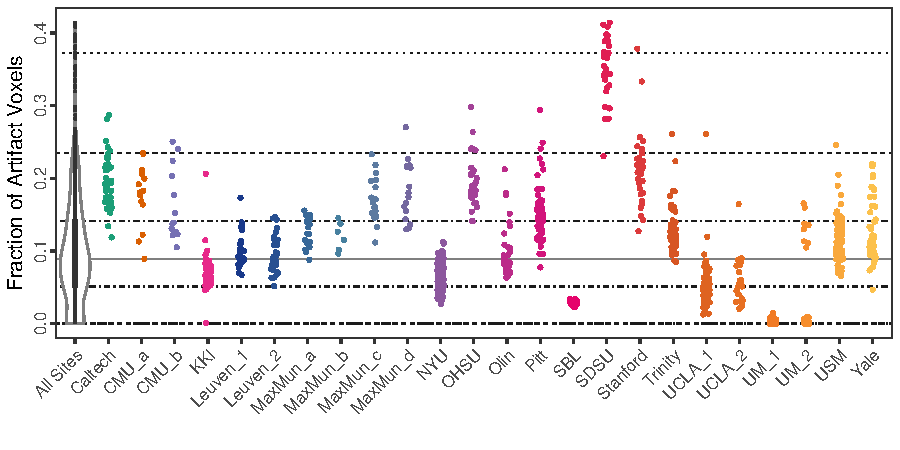
\includegraphics[width=180mm]{data_analysis/abid_anat_spat_Qi1.pdf}
     \caption{Structural MRI fraction of artifact voxels.}
   \end{subfigure}
   \begin{subfigure}[b]{1.0\textwidth}
     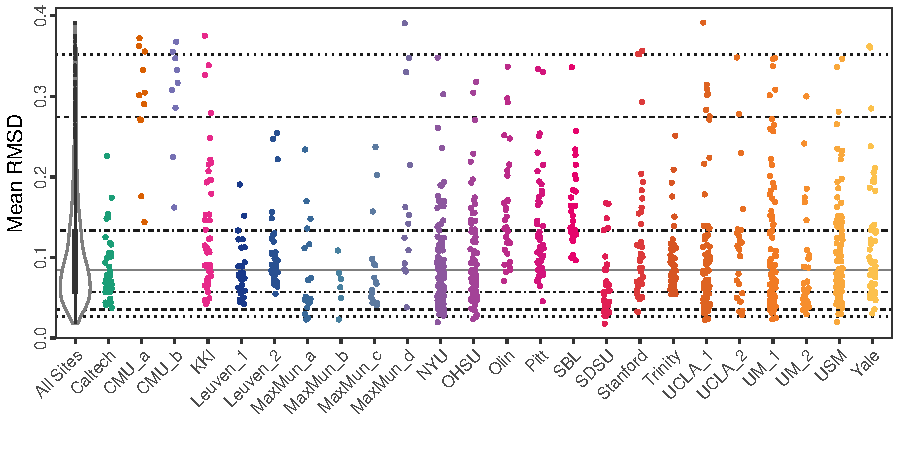
\includegraphics[width=180mm]{data_analysis/abid_func_RMSDMean.pdf}
     \caption{Functional MRI mean root-mean-square deviation.}
   \end{subfigure}
   \caption{Examples of distributions for QAP measures calculated on ABIDE.}
\end{figure}

\begin{figure}[!ht]
  \centering
     \begin{subfigure}[b]{0.4\textwidth}
       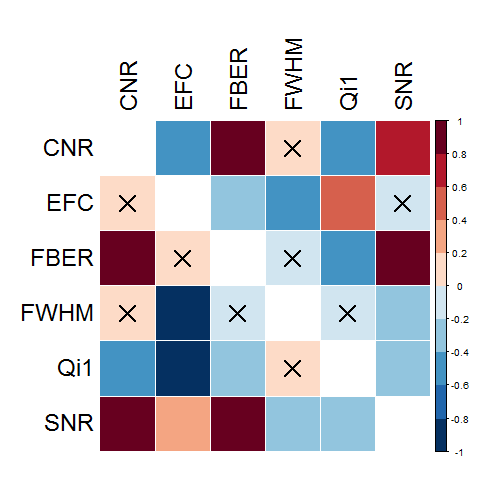
\includegraphics[width=8cm]{fig2_bysite_sig_anat_corrplot}
       \caption{Anatomical measures}
     \end{subfigure}
     \begin{subfigure}[b]{0.4\textwidth}
       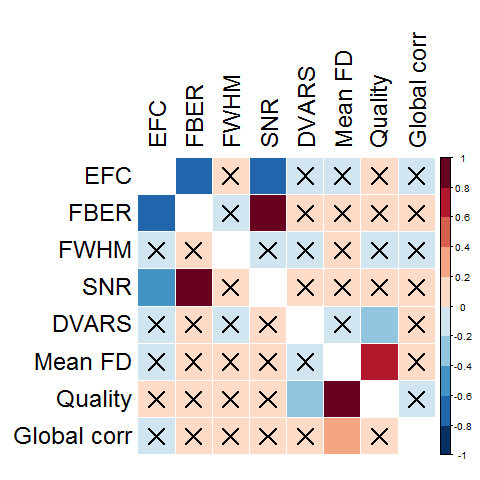
\includegraphics[width=8cm]{fig2_bysite_sig_func_corrplot}
       \caption{Functional measures}
     \end{subfigure}
     \caption{Correlogram of measures: ABIDE in the lower triangular, CoRR in the upper triangular, X=non-significant}
\end{figure}

\begin{figure}[!ht]
  \centering
     \begin{subfigure}[b]{0.4\textwidth}
       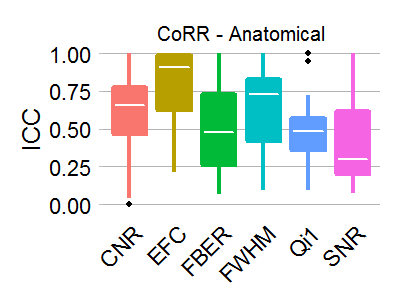
\includegraphics[width=7cm]{fig3_corr_anat_icc_btw}
       \caption{Anatomical measures}
     \end{subfigure}
     \begin{subfigure}[b]{0.4\textwidth}
       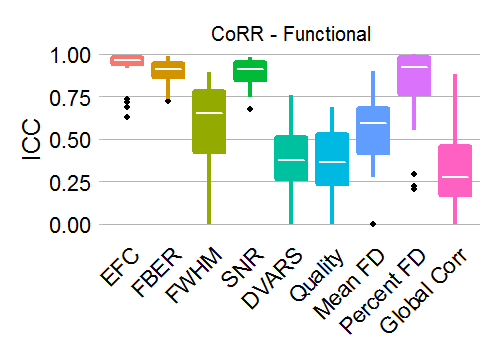
\includegraphics[width=8cm]{fig3_corr_func_icc_btw}
       \caption{Functional measures}
     \end{subfigure}
     \caption{Test re-test of measures for CoRR: Boxplots of ICCs of sites by quality measures.}
\end{figure}

\begin{figure}[!ht]
  \centering
    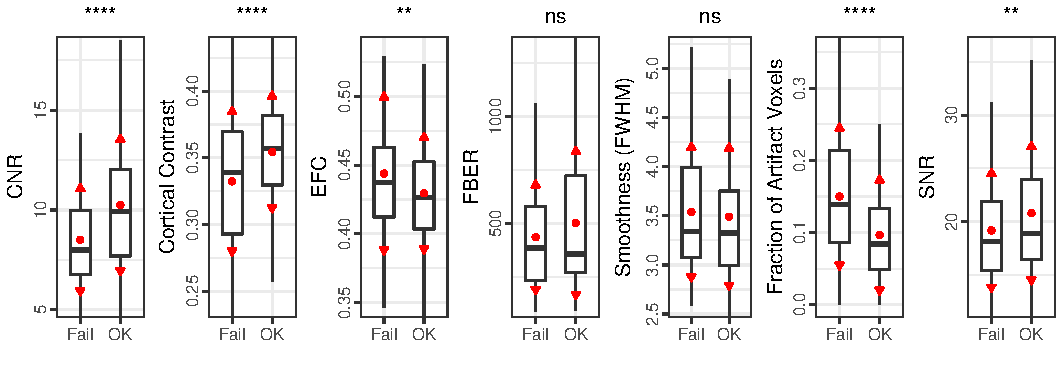
\includegraphics[]{data_analysis/abide_anat_qc}

  \caption{Structural MRI quality measures compared to results of visual inspection.}
\end{figure}

\begin{figure}[!ht]
  \centering
    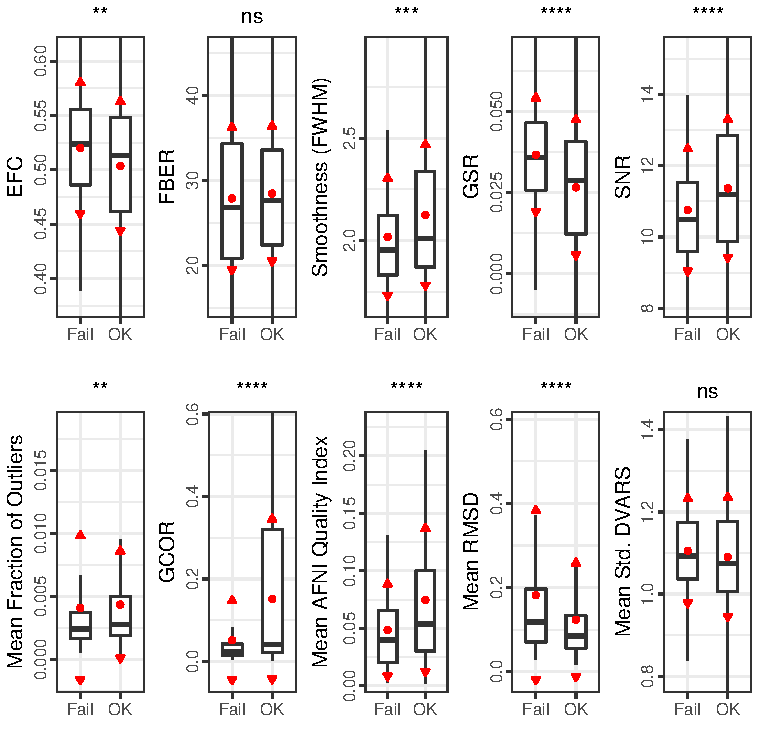
\includegraphics[]{data_analysis/abide_func_qc}
    \caption{Functional MRI quality measures compared to results of visual inspection.}
  \end{figure}
